\chapter{Analysis of the MICEGUT dataset}
\section{Dataset Description}
\textcolor{red}{to be completed}
\begin{figure}[H]
\centering
\fcolorbox{black}{white}{
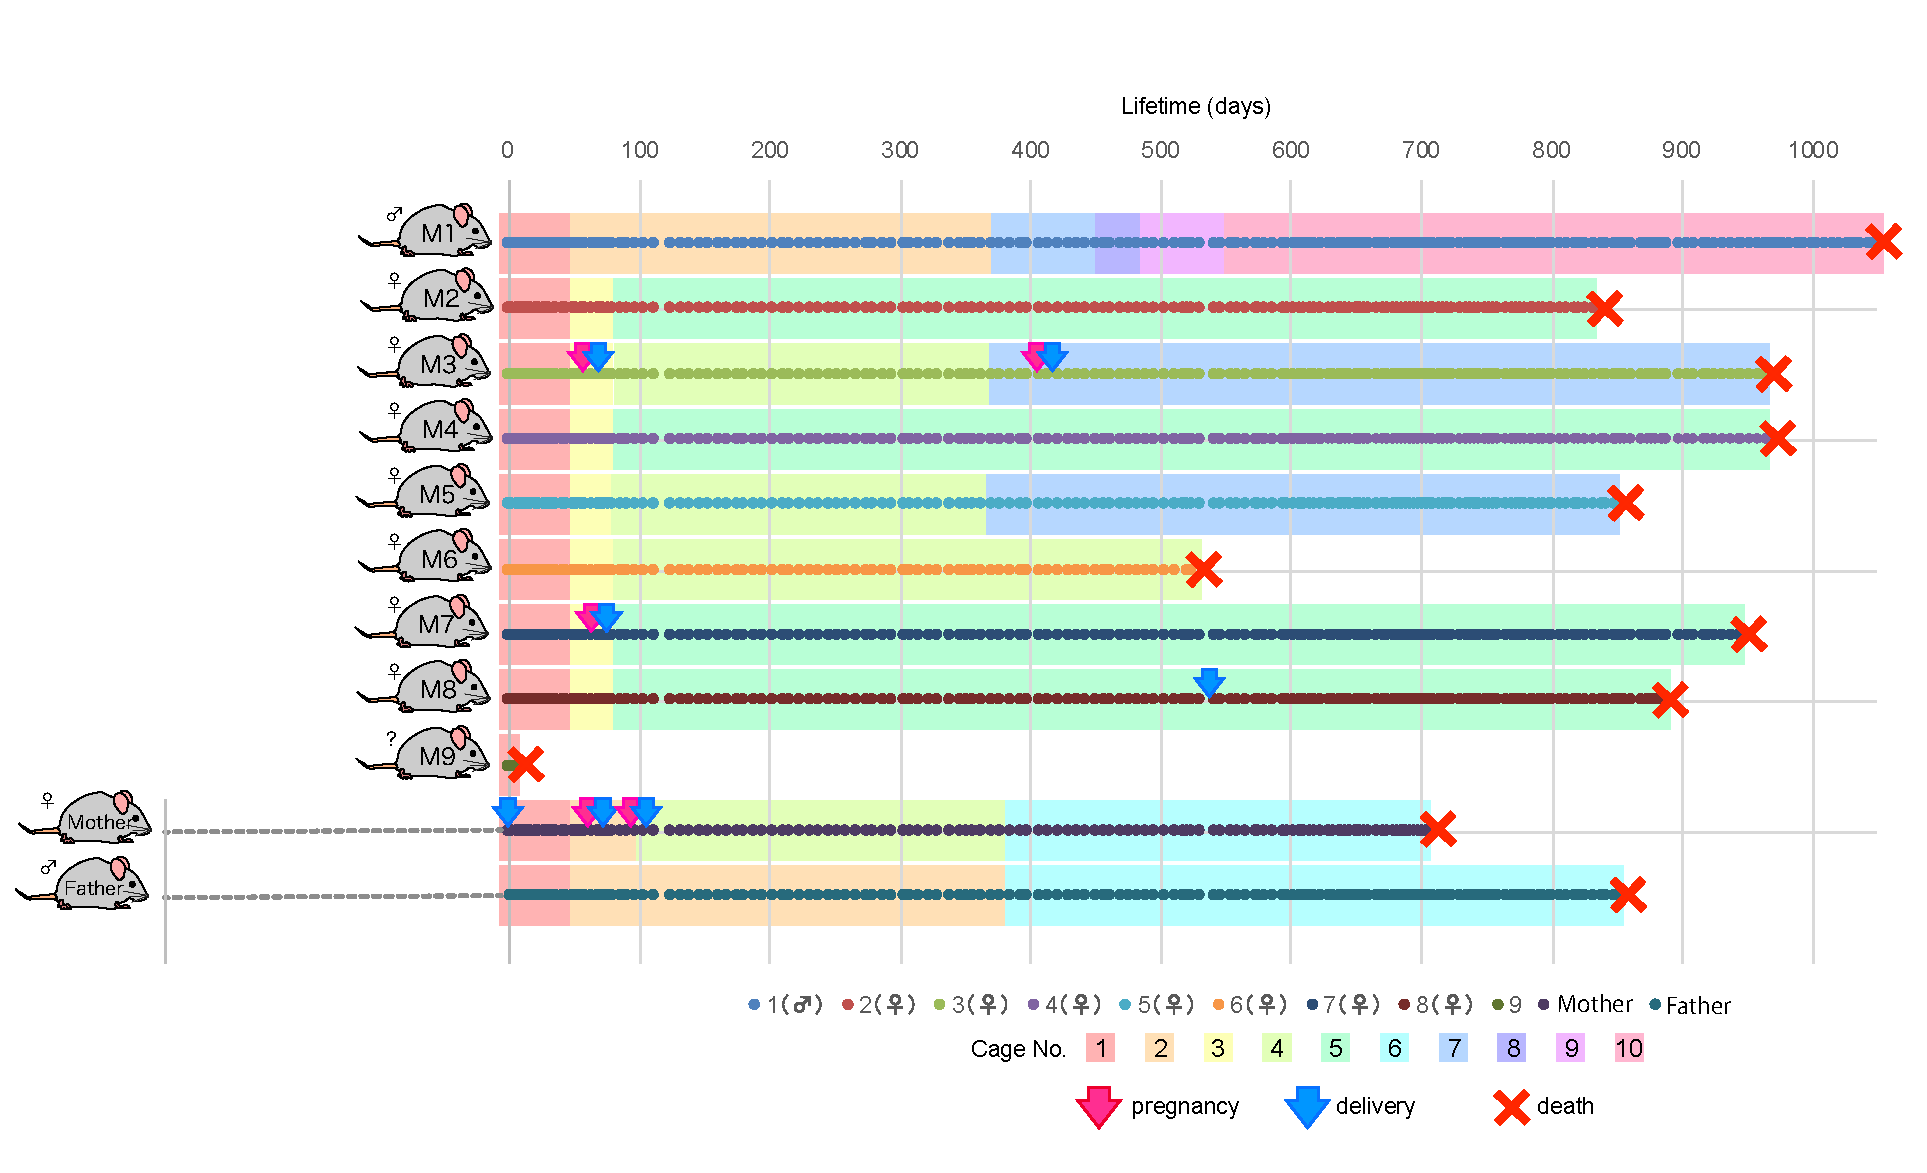
\includegraphics[width = 0.6\linewidth]{figures/chapter_2/fig_data.pdf}
}
\caption{}
\end{figure}

\newpage

\section{Summary Statistics}
\subsection{Rank- Abundance distributions}

\begin{figure}[H]
    \centering
    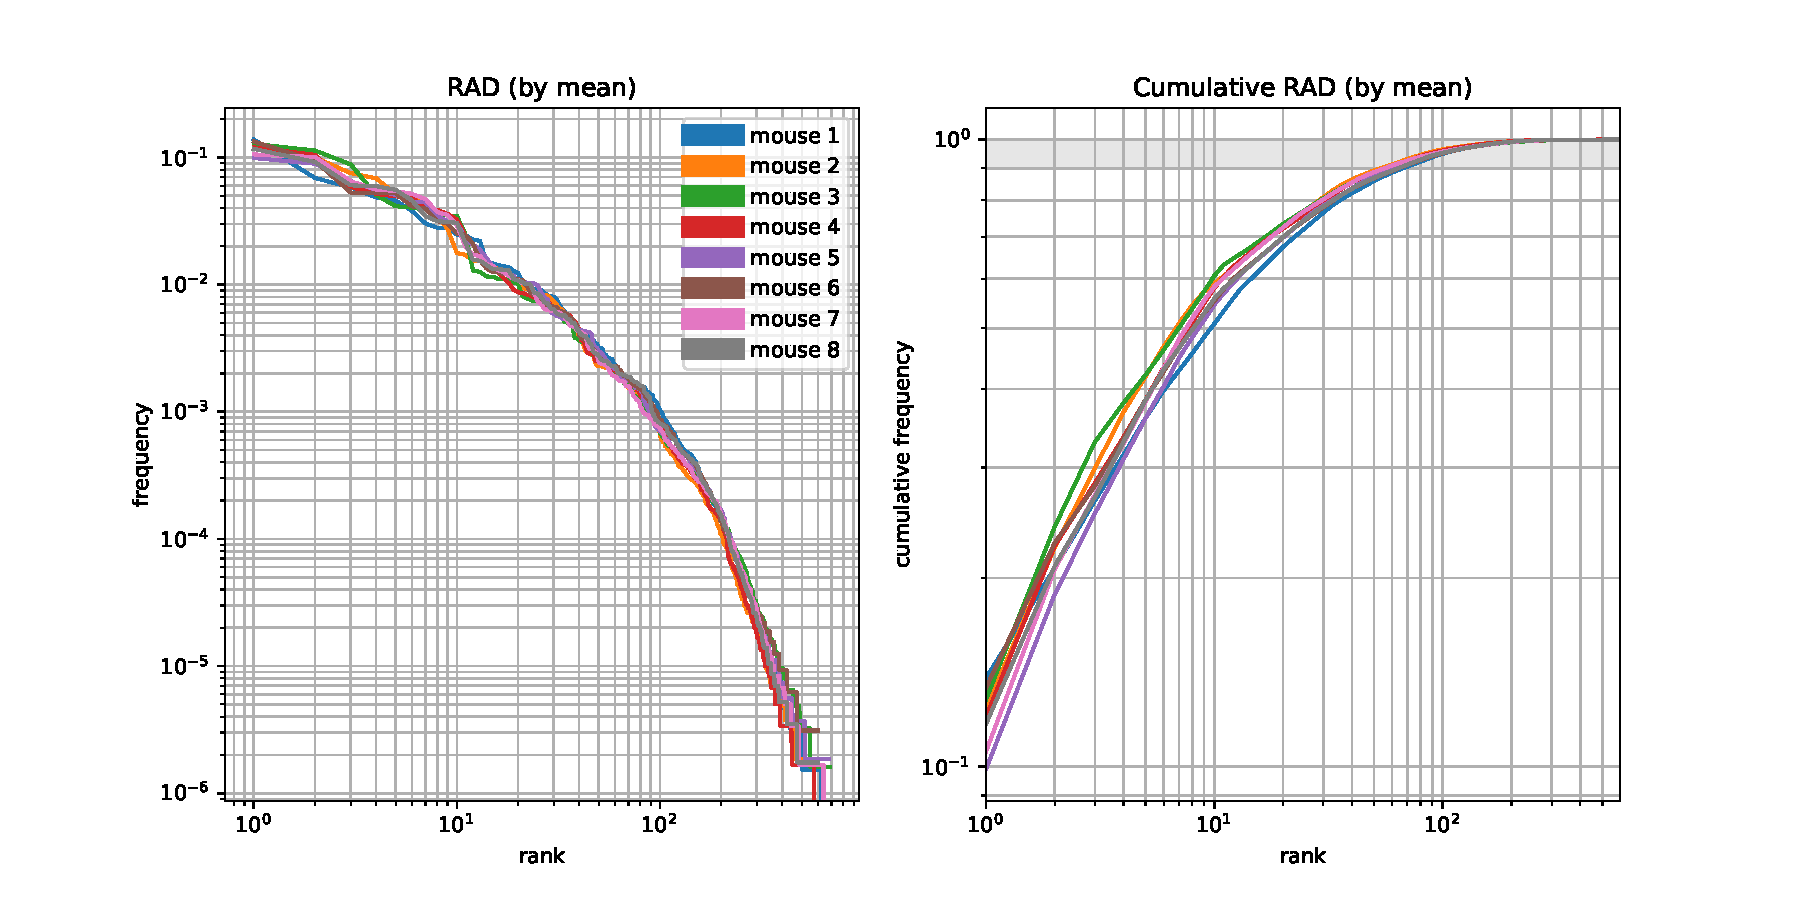
\includegraphics[width=\linewidth]{figures/chapter_2/RAD_mean.pdf}
    \caption{Caption}
    \label{fig:enter-label}
\end{figure}
\subsection{Sample composition across subjects}

\begin{figure}[H]
\centering
\subfigure[]{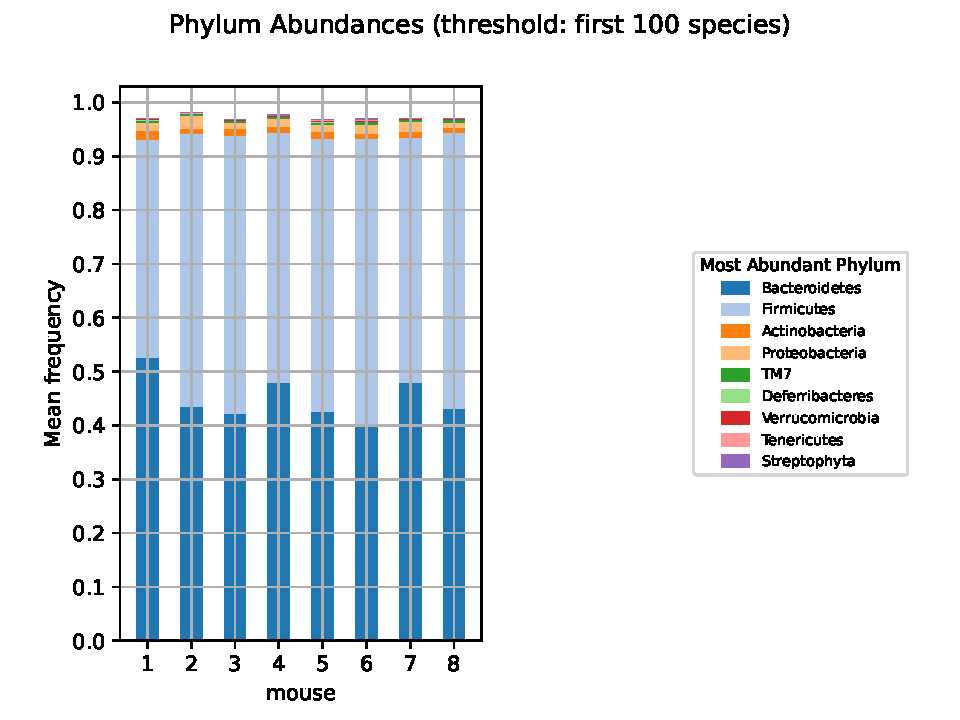
\includegraphics[width=0.48\linewidth]{figures/chapter_2/Phylum_stacked_first_100.pdf}}
\hfill
\subfigure[]{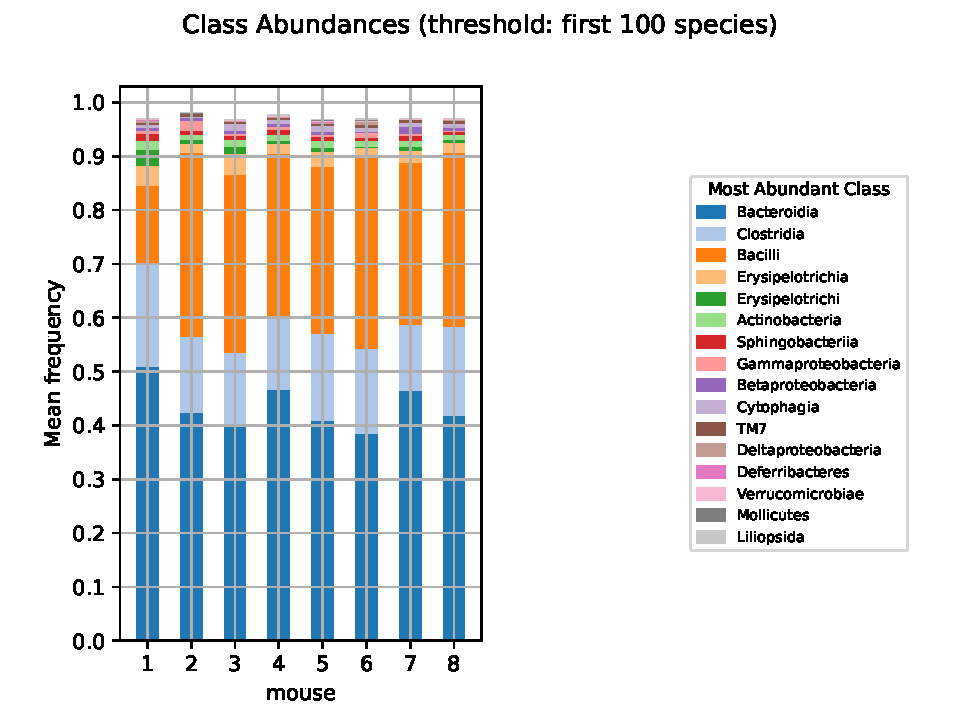
\includegraphics[width=0.48\linewidth]{figures/chapter_2/Class_stacked_first_100.pdf}}
\vspace*{1cm}
\subfigure[]{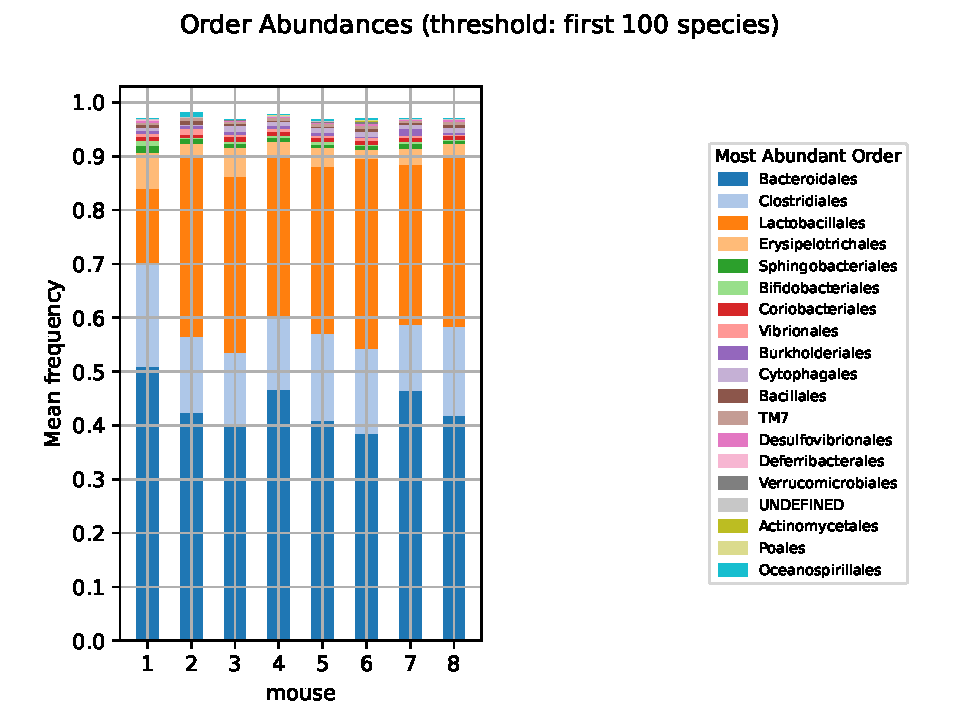
\includegraphics[width=0.48\linewidth]{figures/chapter_2/Order_stacked_first_100.pdf}}
\hfill
\subfigure[]{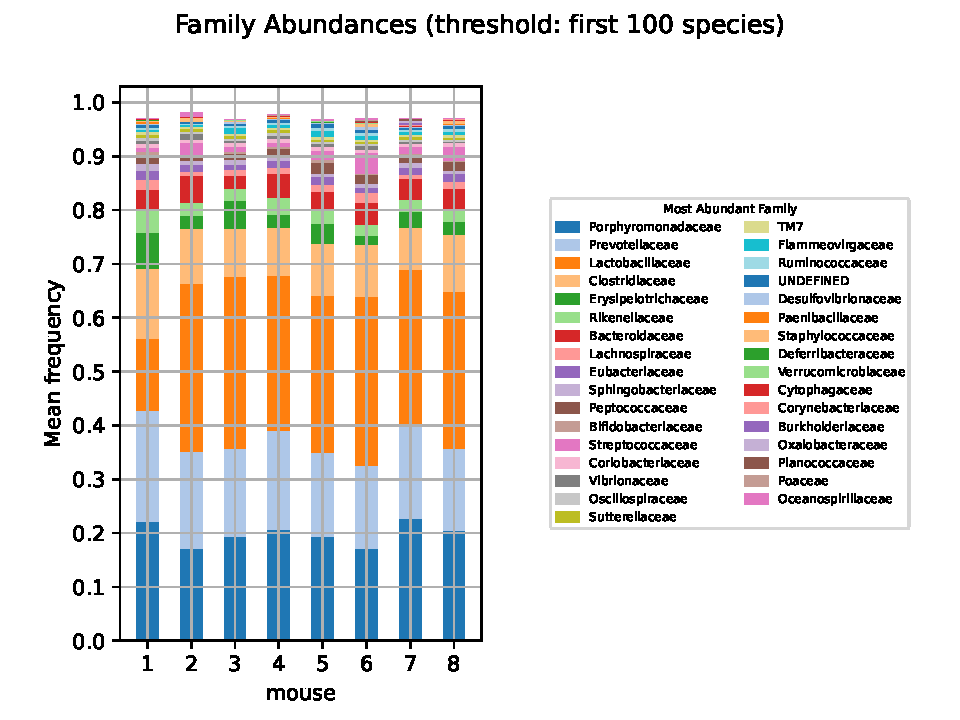
\includegraphics[width=0.48\linewidth]{figures/chapter_2/Family_stacked_first_100.pdf}}
\vspace*{1cm}
\caption{Caption}
\end{figure}

\begin{figure}[H]
    \centering
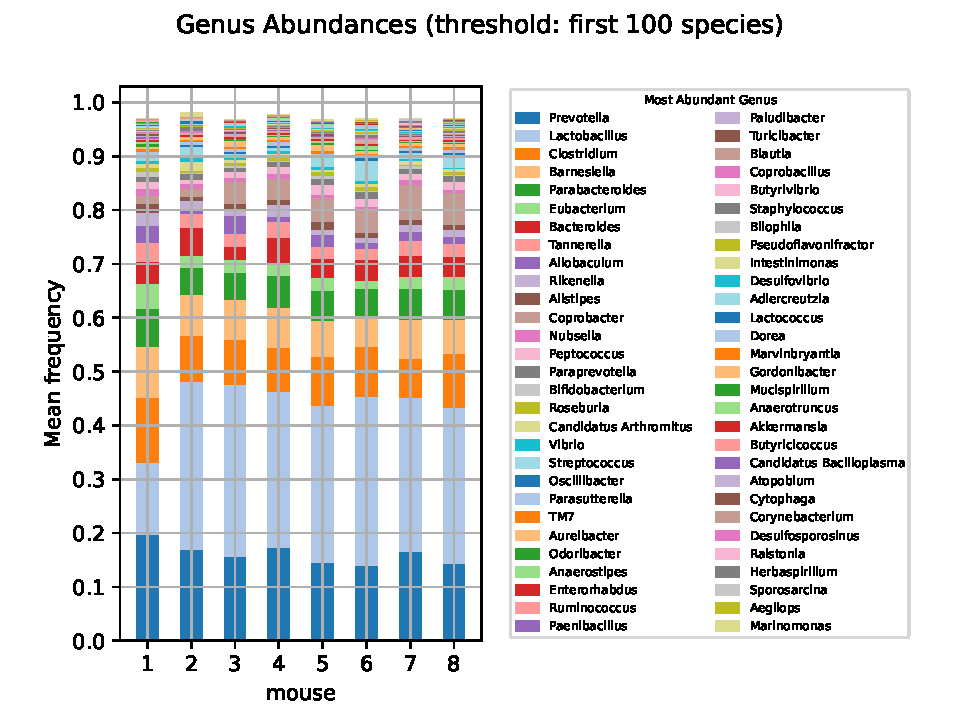
\includegraphics[width=0.9\linewidth]{figures/chapter_2/Genus_stacked_first_100.pdf}

    \label{fig:enter-label}
\end{figure}

\begin{figure}[H]\ContinuedFloat
    \centering
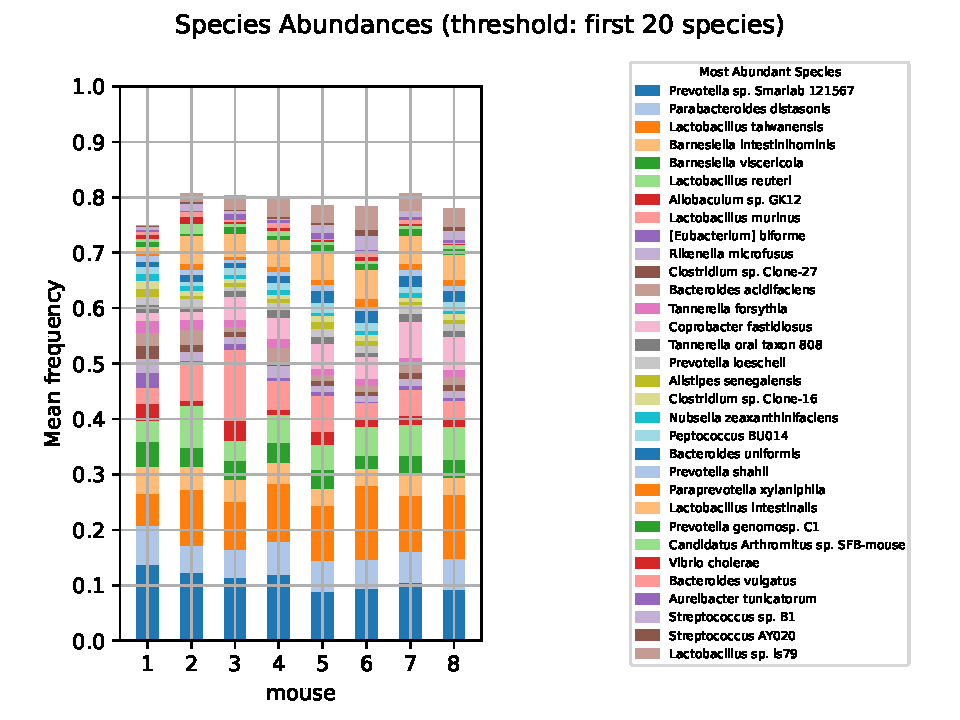
\includegraphics[width=0.9\linewidth]{figures/chapter_2/Species_stacked_first_20.pdf}
    \caption{Taxonomic ranks from bottom to top are:
Species $\subset$ Genus $\subset$ Family $\subset$ Order $\subset$ Class $\subset$ Phylum.}
    \label{fig:enter-label}
\end{figure}

\newpage
\section{Species abundance summary data \textcolor{red}{TO BE COMPLETED}.}



\textcolor{red}{MISSING: Estimation of inter-class and intra-class variance using Linear Mixed Models}
\begin{figure}[H]
    \centering
    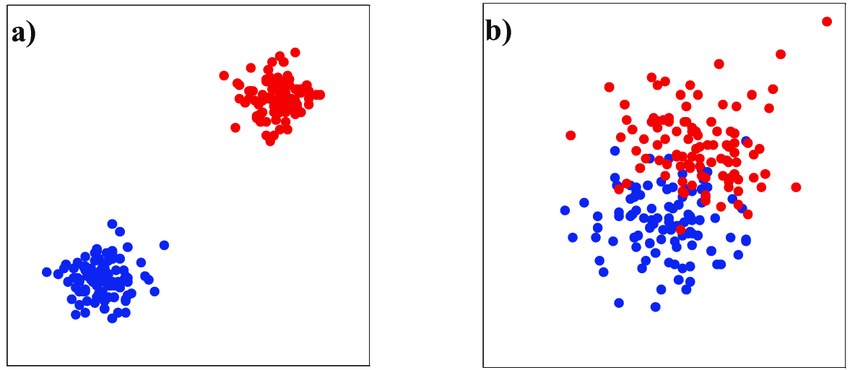
\includegraphics[width=0.5\linewidth]{figures/chapter_2/temp.png}
    \caption{\textcolor{red}{As a reminder.} Inter-class and Intra-class variances concept. a) Low intra-class variance and high inter-class variance: compact well separated clusters. b) High intra-class variance and low inter-class variance: wide clusters without a clear frontier. }
    \label{fig:temp}
\end{figure}

\begin{center}
\begin{longtable}{|l|l|l|l|}
\caption{The table shows the median counts and the mean counts for $136$ species, taken as the union of the $100$ most abundant species by median counts in all mice. The mean counts entry in the table refers to the mean of the mean counts in each mouse.} \label{tab:species_counts} 


\\ \hline \multicolumn{1}{|c|}{\textbf{Rank}} & \multicolumn{1}{c|}{\textbf{Species}} & \multicolumn{1}{c|}{\textbf{Mean counts}} &
\multicolumn{1}{c|}{\textbf{Median counts}}\\
\hline \endfirsthead

\multicolumn{4}{c}% 
{{\tablename\ \thetable{} -- continued from previous page}} \\
\hline \multicolumn{1}{|c|}{\textbf{Rank}} & \multicolumn{1}{c|}{\textbf{Species}} & \multicolumn{1}{c|}{\textbf{Mean counts}} &
\multicolumn{1}{c|}{\textbf{Median counts}}\\
\hline 
\endhead

 \hline 
 \multicolumn{4}{|r|}{Continued on next page}
 \\
 \hline
\endfoot


\hline \hline
\endlastfoot
$1$ & Prevotella sp. Smarlab 121567 & $328.61$ & $320.23$ \\
$2$ & Lactobacillus taiwanensis & $300.42$ & $263.12$ \\
$3$ & Lactobacillus murinus & $170.44$ & $73.31$ \\
$4$ & Parabacteroides distasonis & $167.60$ & $171.12$ \\
$5$ & Lactobacillus reuteri & $153.84$ & $130.00$ \\
$6$ & Lactobacillus intestinalis & $131.43$ & $104.62$ \\
$7$ & Coprobacter fastidiosus & $119.23$ & $93.81$ \\
$8$ & Barnesiella intestinihominis & $111.12$ & $111.52$ \\
$9$ & Barnesiella viscericola & $104.04$ & $103.69$ \\
$10$ & Lactobacillus sp. ls79 & $77.73$ & $61.69$ \\
$11$ & Allobaculum sp. GK12 & $56.04$ & $15.19$ \\
$12$ & Bacteroides acidifaciens & $51.08$ & $32.25$ \\
$13$ & Bacteroides uniformis & $47.93$ & $33.31$ \\
$14$ & Rikenella microfusus & $44.60$ & $37.44$ \\
$15$ & Tannerella forsythia & $44.11$ & $42.38$ \\
$16$ & Peptococcus BU014 & $39.93$ & $27.56$ \\
$17$ & Prevotella loescheii & $39.85$ & $32.38$ \\
$18$ & Tannerella oral taxon 808 & $34.71$ & $30.81$ \\
$19$ & Clostridium sp. Clone-27 & $34.23$ & $13.56$ \\
$20$ & Streptococcus sp. B1 & $33.42$ & $0.00$ \\
$21$ & Paraprevotella xylaniphila & $29.45$ & $19.69$ \\
$22$ & Prevotella genomosp. C1 & $28.07$ & $26.27$ \\
$23$ & Clostridium sp. Clone-16 & $27.81$ & $14.81$ \\
$24$ & [Eubacterium] biforme & $26.30$ & $0.38$ \\
$25$ & Prevotella shahii & $25.90$ & $21.19$ \\
$26$ & Alistipes senegalensis & $25.76$ & $15.12$ \\
$27$ & Nubsella zeaxanthinifaciens & $24.62$ & $23.25$ \\
$28$ & Clostridium sp. Clone-9 & $23.00$ & $11.88$ \\
$29$ & Candidatus Arthromitus sp. SFB-mouse & $22.84$ & $9.00$ \\
$30$ & Prevotella sp. oral taxon 317 & $21.48$ & $20.29$ \\
$31$ & Aureibacter tunicatorum & $19.81$ & $16.12$ \\
$32$ & Clostridium hathewayi & $18.46$ & $10.56$ \\
$33$ & Candidatus Prevotella conceptionensis & $17.26$ & $16.06$ \\
$34$ & Vibrio cholerae & $16.72$ & $0.00$ \\
$35$ & Bacteroides vulgatus & $16.58$ & $9.31$ \\
$36$ & Clostridium sp. ID4 & $15.93$ & $6.06$ \\
$37$ & Parasutterella excrementihominis & $14.24$ & $11.88$ \\
$38$ & TM7 oral taxon 351 & $13.97$ & $12.25$ \\
$39$ & Streptococcus AY020 & $13.06$ & $0.62$ \\
$40$ & Eubacterium sp. F1 & $12.94$ & $7.81$ \\
$41$ & Clostridium sp. ASF502 & $12.62$ & $5.25$ \\
$42$ & Bifidobacterium pseudolongum & $12.18$ & $0.00$ \\
$43$ & Clostridium disporicum & $11.41$ & $2.62$ \\
$44$ & Eubacterium coprostanoligenes & $10.21$ & $6.25$ \\
$45$ & Enterorhabdus caecimuris & $9.82$ & $8.12$ \\
$46$ & [Eubacterium] cylindroides & $9.21$ & $3.75$ \\
$47$ & Eubacterium ventriosum & $8.86$ & $4.69$ \\
$48$ & Staphylococcus aureus & $8.75$ & $0.00$ \\
$49$ & Clostridium indolis & $8.42$ & $3.50$ \\
$50$ & Odoribacter splanchnicus & $8.23$ & $5.00$ \\
$51$ & Prevotella oulorum & $8.11$ & $7.85$ \\
$52$ & Clostridium fusiformis & $8.06$ & $5.00$ \\
$53$ & Clostridium sp. 6-44 & $8.02$ & $5.25$ \\
$54$ & Pseudoflavonifractor capillosus & $7.82$ & $5.94$ \\
$55$ & Prevotella oris & $7.77$ & $7.49$ \\
$56$ & Clostridium sp. Culture-27 & $7.60$ & $3.62$ \\
$57$ & Roseburia sp. 1120 & $7.45$ & $0.25$ \\
$58$ & Oscillibacter valericigenes & $7.27$ & $5.06$ \\
$59$ & Clostridium sp. CRIB & $6.88$ & $2.12$ \\
$60$ & Prevotella IK062 & $6.49$ & $0.38$ \\
$61$ & Clostridium aminophilum & $6.45$ & $2.69$ \\
$62$ & Lactococcus garvieae & $6.09$ & $2.25$ \\
$63$ & Desulfovibrio desulfuricans & $5.88$ & $2.31$ \\
$64$ & Anaerostipes caccae & $5.84$ & $0.62$ \\
$65$ & Ruminococcus lactaris & $5.78$ & $2.88$ \\
$66$ & Paludibacter propionicigenes & $5.62$ & $5.25$ \\
$67$ & Oscillibacter sp. G2 & $5.60$ & $3.38$ \\
$68$ & Clostridium sp. Clone-46 & $5.46$ & $1.62$ \\
$69$ & Adlercreutzia equolifaciens & $5.38$ & $4.25$ \\
$70$ & Clostridium sp. Culture-46 & $5.31$ & $2.38$ \\
$71$ & Clostridium scindens & $5.24$ & $2.25$ \\
$72$ & Clostridium sp. Culture-57 & $5.18$ & $0.81$ \\
$73$ & Dorea longicatena & $5.18$ & $2.56$ \\
$74$ & Alistipes putredinis & $5.12$ & $4.25$ \\
$75$ & Clostridium phytofermentans & $4.96$ & $0.88$ \\
$76$ & Turicibacter sp. LA62 & $4.89$ & $0.62$ \\
$77$ & Clostridium sp. Clone-26 & $4.67$ & $1.75$ \\
$78$ & Clostridium sp. 619 & $4.51$ & $3.25$ \\
$79$ & Clostridium sp. SY8519 & $4.38$ & $1.50$ \\
$80$ & Eubacterium plexicaudatum & $4.33$ & $1.00$ \\
$81$ & Roseburia hominis & $4.28$ & $2.25$ \\
$82$ & Clostridium sp. Culture-23 & $4.26$ & $2.06$ \\
$83$ & Clostridium sp. Clone-44 & $4.24$ & $1.75$ \\
$84$ & Intestinimonas butyriciproducens & $4.14$ & $2.31$ \\
$85$ & Coprobacillus sp. $8$\_$2$\_$54$BFAA & $4.13$ & $1.50$ \\
$86$ & Clostridium sp. 826 & $4.05$ & $1.62$ \\
$87$ & Lactobacillus johnsonii & $3.91$ & $2.00$ \\
$88$ & Ruminococcus flavefaciens & $3.66$ & $1.31$ \\
$89$ & Clostridium sp. cTPY-12 & $3.60$ & $1.12$ \\
$90$ & Clostridium sp. ASF356 & $3.56$ & $1.50$ \\
$91$ & Parabacteroides merdae & $3.29$ & $2.50$ \\
$92$ & [Clostridium] cocleatum & $3.19$ & $0.25$ \\
$93$ & Gordonibacter pamelaeae & $3.15$ & $2.56$ \\
$94$ & Akkermansia muciniphila & $3.15$ & $0.62$ \\
$95$ & Roseburia sp. 499 & $2.92$ & $0.88$ \\
$96$ & Clostridium sp. YIT 12070 & $2.70$ & $0.19$ \\
$97$ & Clostridium clostridioforme & $2.66$ & $1.12$ \\
$98$ & Clostridium saccharolyticum & $2.47$ & $1.19$ \\
$99$ & Clostridium sp. Clone-47 & $2.28$ & $0.88$ \\
$100$ & Atopobium parvulum & $2.26$ & $0.75$ \\

\end{longtable}
\end{center}

As one can see by looking at the table \ref{tab:species_counts}, there are some species which are high in mean abundance while low in median abundance: these are species which are present during the first days of mice's lives and then drop rapidly to zero counts, meaning they go extinct or very rare. Some examples of such species are \textit{Streptococcus AY020}, \textit{Vibrio cholerae}, \textit{Eubacterium biforme}, \textit{Candidatus Arthromitus sp. SFB-mouse}, \textit{Streptococcus sp. B1} [Figure: \ref{fig:rare_species}]. In particular, some strains of \textit{Vibrio cholerae} are pathogenic and responsible for cholera disease. The data shows in that this bacterium is initially present in neonatal mice and then gets suppressed.  "Candidatus Arthromitus" sp. strain SFB-mouse-NL (SFB, segmented filamentous bacteria) is a commensal bacterium necessary for inducing the postnatal maturation of homeostatic innate and adaptive immune responses in the mouse gut \parencite{candidatus_arthromitus}.

\begin{figure}[H]
    \centering
    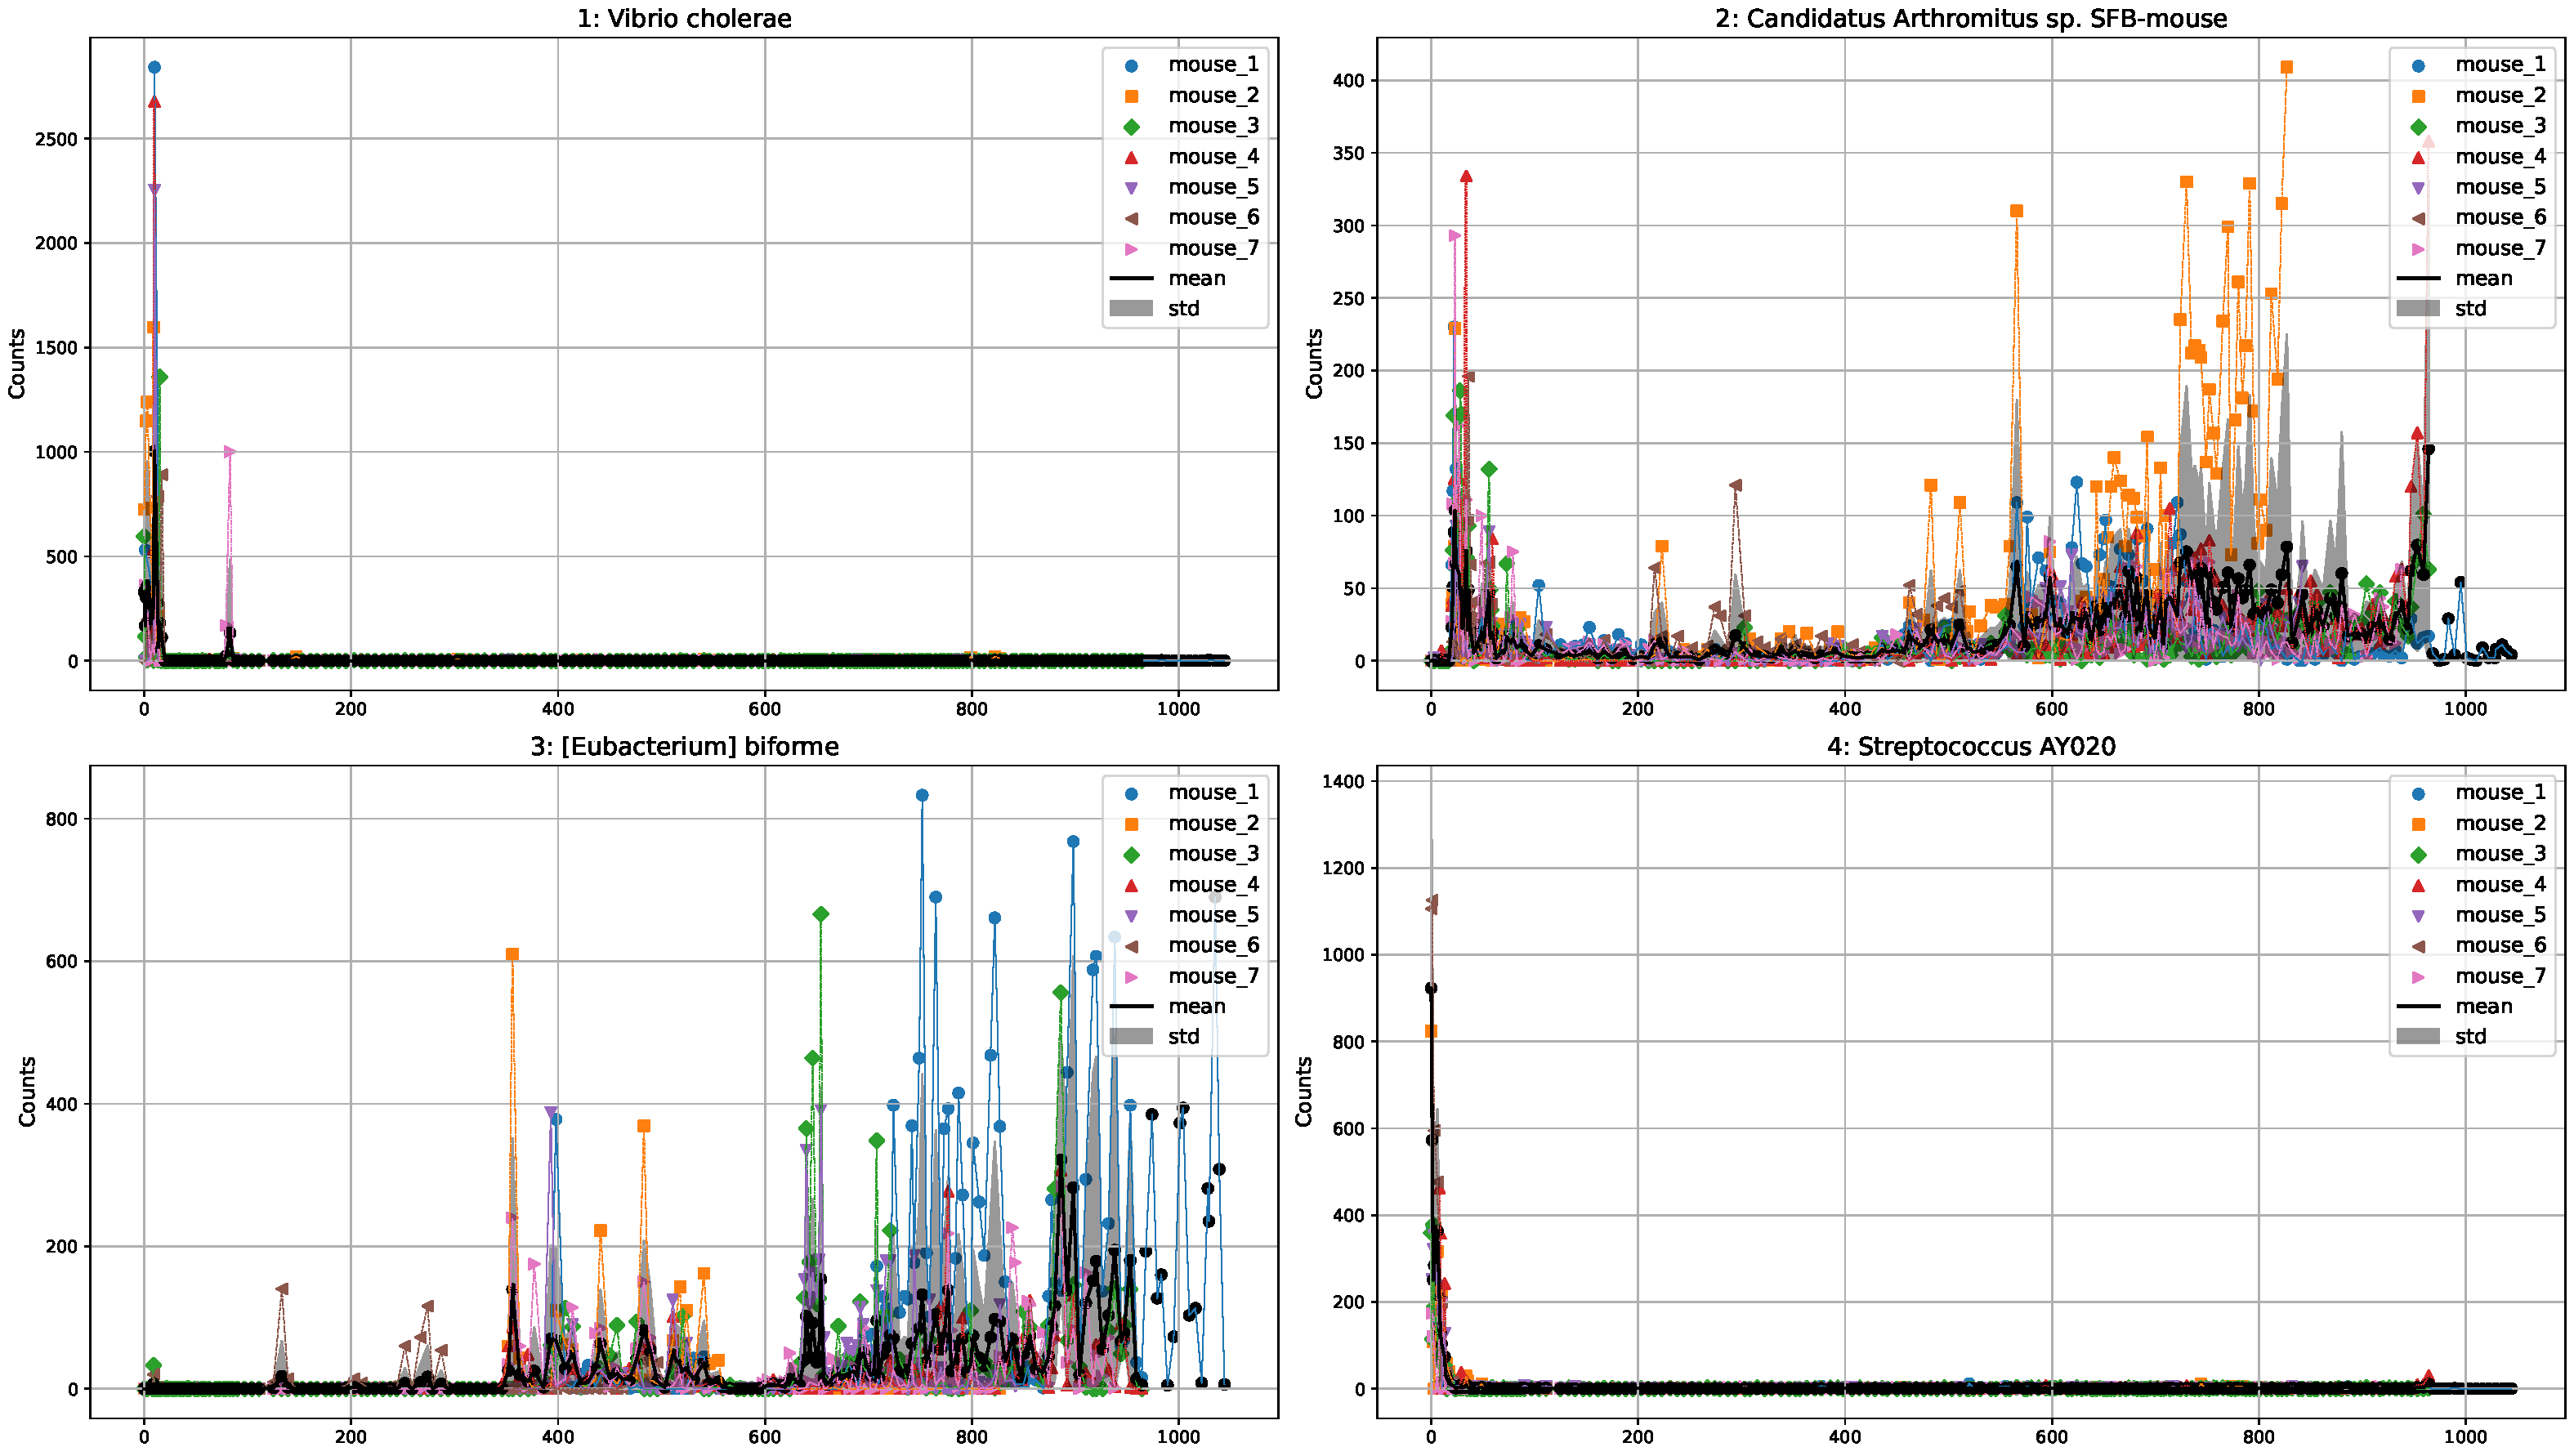
\includegraphics[width=\linewidth]{tables/chapter_2/rare_mean_species.pdf}
    \caption{Caption}
    \label{fig:rare_species}
\end{figure}
\newpage
\section{Gallery of timeseries plots.}


